\documentclass[10pt,landscape]{article}
% \pagestyle{headings}
\usepackage{multicol}
\usepackage[landscape]{geometry} 
\usepackage{amsfonts}
\usepackage{amssymb}
\usepackage{amsmath}
\usepackage{latexsym}
\usepackage{enumerate}
\usepackage{verbatim}
\usepackage{multirow}
\usepackage[lofdepth,lotdepth]{subfig}
\usepackage[pdftex]{graphicx}
\setlength{\parindent}{0pt}
\setlength{\parskip}{0pt plus 0.5ex}
% \setlength{\parskip}{1ex plus 0.5ex minus 0.2ex}
\setlength{\topmargin}{-1.35in}
\setlength{\textheight}{8in}
\setlength{\oddsidemargin}{-0.75in}
\setlength{\evensidemargin}{-0.75in}
\setlength{\textwidth}{10.5in}
% \setlength{\baselineskip}{-1pt}
% \renewcommand{\baselinestretch}{0.5}

\makeatletter
\renewcommand{\section}{\@startsection{section}{1}{0mm}%
  {-1ex plus -.5ex minus -.2ex}%
  {0.5ex plus .2ex}%x
  {\normalfont\large\bfseries}}
\renewcommand{\subsection}{\@startsection{subsection}{2}{0mm}%
  {-1explus -.5ex minus -.2ex}%
  {0.5ex plus .2ex}%
  {\normalfont\normalsize\bfseries}}
\renewcommand{\subsubsection}{\@startsection{subsubsection}{3}{0mm}%
  {-1ex plus -.5ex minus -.2ex}%
  {1ex plus .2ex}%
  {\normalfont\small\bfseries}}
\renewcommand{\thesection}{\Roman{section}}
\makeatother

\newcommand{\ps}{\ \vspace{0.05in}}
\newcommand{\dg}{$^\circ$ }
\newcommand{\img}[1]{\includegraphics[scale=0.5]{#1}}

% Don't print subsection numbers
\setcounter{secnumdepth}{1}

\thispagestyle{empty} 

\begin{document}


\begin{multicols*}{3}
\raggedright
\section*{Synthesis Study Guide - Feynman Liang\\
  CHEM231 - Spring 2012\\
  Amherst College}
  
  \begin{scriptsize}
    
    \section{Substitution}

    \begin{itemize}
    \item S$_n$2 - single step, 100\% inversion, \textbf{1\dg electrophile} (else E2 dominates),
      \textbf{DMSO or acetone} solvent (polar aprotic)
    \item S$_n$1 - rate determined by carbocation formation, shifts possible, racemic
      product, \textbf{3\dg electrophile} (E1 will always be present), \textbf{H$_2$O or
        compatible (will not generate other products) ROH} solvent (polar protic)
    \item Good nucleophile (sterically unhindered, basic)
    \item Good leaving group (strong conj. acid)
    \end{itemize}


    \subsection{Making alkyl halides (R-X)}

    \begin{itemize}
    \item \textbf{Alcohol using acid} from R-OH$_2^+$, protonation followed by halide
      substitution of H$_2$O$^+$:
      \begin{itemize}
      \item[] \img{makingrx1.png}
      \item S$_N$1 unless 1\dg. S$_N$2 competes with elimination (unhindered substrate and
        good Nu to favor substitution)
      \end{itemize}
    \item \textbf{Alcohol using TsCl}, tosylate (OTs) L-group instead of OH$_2^+$:
      \img{makingrx2.png}
      \begin{itemize}
      \item Two-step process (1. convert, 2. substitute)
      \item Could have also eliminated OTs after step 1 in E2 (Saytzeff's rule)
        \img{elimot.png}
      \end{itemize}
    \item \textbf{Alcohol using SOCl$_2$}:
      \begin{itemize}
      \item[] \img{makingrx3.png}
      \item One-step process, hydroxyl attacks S and SO$_2$ + Cl$^-$ is displaced by
        Cl$^-$ nucleophilic substitution
      \item Pyridine should be used to neutralize HCl
      \item Will also convert all COOH to COCl
      \end{itemize}
    \end{itemize}

    \subsection{Williamson ether synthesis (R-O-R')}
    
    \begin{itemize}
    \item[] \img{williamson.png}
    \item S$_N$2, inversion of configuration
    \item Alkoxide (RO$^-$) formed by ROH + NaH (Na$^+$ $^-$OR)
    \item Electrophile must be 1\dg, E2 predominates 2\dg and 3\dg
    \item Intramolecular forms cyclic ethers, bridged rings, epoxides, etc.
    \item Unlike acid Cl or Fisher esterification, does not require carbonyl group
    \end{itemize}

    \subsection{Alkylation of amines (R$_x$-NH$_x$)}

    \begin{itemize}
    \item[] \img{aminealkylation.png}
    \item S$_N$2, inversion
    \item Possible deprotonation of amide product by NH$_3\rightarrow$NH$_4^+$ may result
      in multiple alkylations
    \item 1\dg substrate required (or else E2 predominates)
    \end{itemize}

    \subsection{Other nucleophiles for C-C bond making}
    
    \begin{itemize}
    \item \textbf{Cyanide ($^-$CN)}::
      \begin{itemize}
      \item[] \img{cc1.png}
      \item Moderate base/good Nu, favors S$_N$2
      \item Can hydrolyze -CN to COOH
      \end{itemize}
    \item \textbf{Acetylide anion ($^-$:C$\equiv$CR)}:
      \begin{itemize}
      \item[] \img{cc2.png}
      \item Anion generated from deprotonation (pKa$\approx$25), (Na$^+$)$^-$NH2 is
        good base for this
      \item Strong Nu, S$_N$2
      \end{itemize}
    \end{itemize}

    \section{Alkene addition}
    
    \begin{itemize}
    \item Formed by \textbf{eliminaton}:
      \begin{itemize}
      \item Alcohol dehydration: R-R-OH + H$_3$O$^+$ + $\triangle$ $\rightarrow$ R=R + 2
        H$_2$O (reversed using strong base )
      \item \textbf{E2} occurs between anti-periplanar H and L, favored over S$_N$2 with strong
        base, steric hindrance, higher temp
      \item \textbf{E1 }has unselective stereochemistry, always accompanies S$_N$1
      \item Regiochemistry follows \textbf{Saytzeff's rule}: product favors more highly substituted alkene
        b/c hyperconjugation of transition state
      \end{itemize}
    \item General Rules for Addition:
      \begin{itemize}
      \item Markovnikov's rule: positively charged adding reagant (usually H$^+$) attaches
        to alkene to create more stable carbocation intermediate (to less substituted C so
        the carbocation has + charge on higher substituted C)
      \item Dimerize/polymerize: the carbocation formed can be attacked by the
        nucleophilic $\pi$-bond
      \item Br$_2$ and Cl$_2$ form trans-dihalides (through halonium ion). Halonium can
        also be attacked by other Nu (\textbf{Note:} Nu will attack carbon with more
        positive charge, which is usually more substituted one b/c hyperconjugation
        stabilized)
      \end{itemize}
      
    \end{itemize}

    \subsection{Hydrogenation}

    \begin{itemize}
    \item[] \img{alkene-hydrog.png}
    \item H$_2$ gas and metal catalyst (Pd/C), rxn on surface of metal
    \end{itemize}

    \subsection{Hydroboration/oxidation}

    \begin{itemize}
    \item[] \img{hbor1.png}
    \item Two-step anti-Markovnikov syn-addition of water across double bond with no
      rearrangements 
    \item[1. ] Hydroboration:
      \begin{itemize}
      \item[] \img{hbor2.png}
      \item Concerted (single step, no rearrangements of carbocation possible)
      \item Regioselective: BH$_2$ adds to less substituted end (Markovnikov's rule)
      \item Syn-addition (H and BH$_2$ on same face of alkene) consistent w/ concerted
      \item Product R-BH$_2$ reacts 3x more until trialkylborane (BR$_3$) is formed
      \end{itemize}
    \item[2. ] Oxidation of alkylboranewith peroxide:
      \begin{itemize}
      \item[] \img{hbor3.png}
      \item BR$_3$ attacked by $^-$OOH to form B(OR)$_3$, which is then substituted by
        $^-$OH
      \item \textbf{Stereochemistry of carbon with BH2 is retained}
      \end{itemize}
    \end{itemize}

    \subsection{Oxymercuration/reduction}

    \begin{itemize}
    \item[] \img{omer1.png}
    \item Three-step Markovnikov anti-addition of water across double bond with no
      rearrangements
    \item Preferred way (vs acid catalyzed) to hydrate alkene
    \item[1. ] Oxymercuration:
      \begin{itemize}
      \item[] \img{omer2.png}
      \item Mercurinium prevents rearrangements, can form on both faces of alkene
      \end{itemize}
    \item[2. ] Opening of mercurinium ion:
      \begin{itemize}
      \item[] \img{omer3.png}
      \item If not symmetric,  $^-$OH adds to more substituted end (b/c more + charge, think
        halonium attack)
      \end{itemize}
    \item[3. ] Reduction:
      \begin{itemize}
      \item[] \img{omer4.png}
      \item Stereochemistry of reduction is random
      \end{itemize}
    \end{itemize}

    \subsection{Alkene epoxidation (alkene $\rightarrow$ epoxide $\rightarrow$
      1-hydroxy,2-substituted)}

    \begin{itemize}
    \item[] \img{epox1.png}
    \item Single-step formation of epoxide (3-membered ring with O), stereochemistry preserved
    \item Epoxides can be opened by Nu to give alcohol:
      \begin{itemize}
      \item[] \img{epox2.png}
      \item Under non-acidic, Nu attacks less-hindered carbon (think S$_N$2) with inversion
      \item Examples of possible Nu: NC$^-$, HS$^-$, I$^-$, RC$\equiv$C$^-$,
        HO$^-$, RO$^-$, Br$^-$, N$_3$$^-$, NH$_3$, organometals, metal hydrides
      \end{itemize}
    \end{itemize}
    
    \subsection{Ozonolysis (alkene $\rightarrow$ two carbonyls)}

    \begin{itemize}
    \item Ozone cleavage of alkene to generate two separate carbonyls:\\
      \img{ozon1.png}
    \item Alkene $\rightarrow$ Molozonide (unstable) $\rightarrow$ Ozonide:\\
      \img{ozon2.png}
    \item Reduction of Ozonide (commonly Me$_2$S) yields two carbonyls:\\
      \img{ozon3.png}
    \item Note: reaction can also be intermolecular, resulting in only one dicarbonyl
      product
    \end{itemize}

    \subsection{Dihydroxylation (alkene $\rightarrow$ 1,2-diol)}

    \begin{itemize}
    \item Alkene oxidation to 1,2-diol using KMnO$_4$ or OsO$_4$\\
      \img{dihy1.png}
    \item Concerted first step forms unstable intermediate (followed by removal of MnO$_2$)\\
      \img{dihy2.png}
    \item OsO$_4$ is similar. Intermed can be isolated but generally transformed to
      diol with sodium sulfite:\\
      \img{dihy3.png}
    \item Use OsO$_4$ if you do not want to oxidize aromatic alkyls to COOH
    \end{itemize}
    
    \section{EAS}
    
    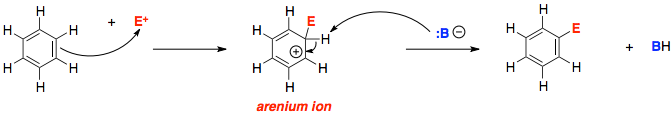
\includegraphics[scale=0.35]{easmech.png}
    
    \begin{itemize}
    \item Res. stabilized arenium intermed, substitution trumps addition b/c deprotonation
      restores aromaticity
    \item To determine rate and directing effects  of substituents, compare stability (res,
      hyperconj, induct) of possible arenium intermed (Hammond Postulate)
    \item In general, EDG = o/p activating and EWG = m deactivating (\textbf{exception}: halogens
      are o/p deactivating due to induct > res,)
    \item Not limited to just benzene, EAS also possible on:
      \begin{tabular}{cc}
        \img{pyridine.png} & \img{pyrrole.png}\\
        Pyridine & Pyrrole
      \end{tabular}
    \end{itemize}

    \subsection{Diazonium ion (R-NO$_2$ $\rightarrow$ R-NH$_2$ $\rightarrow$
      R-N$^+\equiv$N)} 
    
    \begin{itemize}
    \item Nitro (NO$_2$, meta directing) can be reduced to amino (NH$_2$, o/p directing)
      \img{diaz1.png}\\
    \item \textbf{Careful!} H$_2$ with Pd/C \emph{will also hydrolyze alkenes}
    \item Amine (R-NH$_2$) can be converted to diazonium ion (R-N$^+\equiv$N), which can
      be further substituted through S$_N$1:\\
      \img{diaz2.png}
    \end{itemize}

    \subsection{Reactions from diazonium (R-N$^+\equiv$N $\rightarrow$ R-X)}

    \begin{itemize}
    \item \textbf{Sandmeyer reaction}: Cuprous salt substitution of diazonium ion (see
      summary for reactants):\\
      \img{sandmeyer.png}
    \item Can also treat diazonium with KI to form R-I
    \item Can also hydrolize with H$_3$O$^+$ to form R-OH
    \end{itemize}

    \subsection{Clemmensen reduction of acyl to alkyl}
    
    \begin{itemize}
    \item[] \img{clemm.png}
    \item Requires strongly acidic conditions. Allows for EAS alkylation using acyl groups
      (which won't undergo carbocation shifts and can be reduced to alkyl) and many other
      pathways.
    \end{itemize}

    \subsection{Oxidation of alkyl to COOH}
    
    \begin{itemize}
    \item[] \img{alkylox.png}
    \item Reverse of Clemmenson, basic rxn conditions, mechanism likely through benzylic
    \end{itemize}

    \subsection{Summary of EAS}
    
    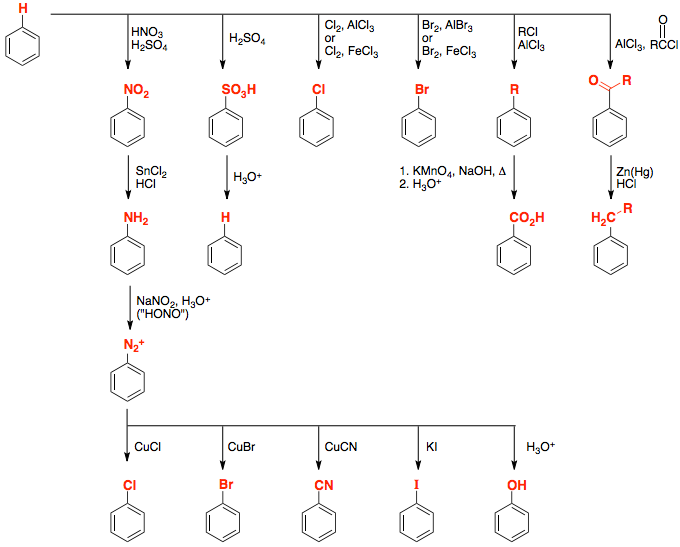
\includegraphics[scale=0.36]{eas.png}
    
    \section{Carbonyl chemistry}

    \subsection{Nucleophilic attack at carbonyl}
    \begin{itemize}
    \item To determine reactivity, look at stability (hyperconj, res, inductive) of charge
      separated form of carbonyl: \\
      \img{carbonylres.png}
    \item Reactivity: Acid Cl $>$ Aldehyde $>$ Ketone $>$ Ester $>$ Amide
    \item Aldehydes and ketones undergo \textbf{addition} (because no L-group):\\
      \img{carbonyladd.png}
    \item Acid Cl, ester, amide, carboxylic acids undergo \textbf{substitution}:\\
      \img{carbonylsub.png}
    \item Nitriles react similarly to carbonyl:\\
      \img{nitrile.png}
    \end{itemize}

    \subsection{Addition reactions (ketones/aldehydes)}

    \begin{itemize}
    \item \textbf{Hydration/dehydration}: carbonyl $\rightarrow$ 1,1-diol, acid or base
      catalyzed\\
      \img{hydrate1.png}
    \item \textbf{Acetal formation}, carbonyl $\rightarrow$ acetal, acid catalyzed\\
      \img{acetal2.png}
      \begin{itemize}
      \item Hemiacetal intermed. unstable, only cyclic can be isolated 
      \item EQ driven towards acetal w/ excess alcohol or removing H$_2$O
      \item Reverse is \textbf{acetal hydrolysis}, acid catalyzed
      \item No rxn in basic conditions (can't eliminate from hemiacetal)
      \end{itemize}
    \end{itemize}

    \subsection{Addition w/ nitrogen nucleophile}
    
    \begin{itemize}
    \item All drived forwards by removing H$_2$O, reverse is hydrolysis
    \item \textbf{Imine formation} from primary amine, netural conditions:
      \img{nnuc1.png}
      \begin{itemize}
      \item pH$\geq$4 prevent protonation of amine to ammonium  hydrolysis, pH$\leq$6 to prevent
        deprotonation to unreactive carboxylate ion
      \item \textbf{Reductive amination} can be achieved by reducing the resulting imine
        (NaBH$_4$):\\
        \img{redamine.png}
      \end{itemize}
    \item \textbf{Enamine formation} from secondary amine (identical until last step):

      \img{enamine.png}

    \item \textbf{Tertiary amines are unreactive }b/c can't stabilize + charge
    \end{itemize}

    \subsection{Substitution reactions (acid Cl, ester, amide, COOH)}
    
    \begin{itemize}
    \item \textbf{Fischer esterification}, RCO(OH) $\rightarrow$ RCO(OR') (Note: should
      only use over SOCl$_2$ activation if multiple COOH sites):
      \img{fischer.png}
      \begin{itemize}
      \item Acid catalyzed (K$\approx$1), driven towards ester w/ excess RCOOH or R'OH or
        removing H$_2$O
      \item No reaction in base (deprotonate to carboxylate)
      \item Reverse is \textbf{ester hydrolysis} (RCO(OR') $\rightarrow$ RCO(OH)), acid catalyzed but
        base induced (deprotonate to carboxylate)
      \item \textbf{Transesterification} (RCOOR' + R''OH $\rightarrow$ RCOOR'' + R'OH):
        \img{transester.png}
      \end{itemize}
    \item \textbf{Amide hydrolysis} substitutes amide (-NH2) with (-OH):
      \img{amidehydr.png}
      \begin{itemize}
      \item Acid (NH$_2$R reacts with acid to form NH$_4^+$) and base (NHR reacts with COOH to form
        carboxylate) induced
      \end{itemize}
    \item \textbf{Activating COOH $\rightarrow$ acid Cl with SOCl$_2$} converts COOH to most
      reactive acid Cl:
      \img{acidcl.png}
      \begin{itemize}
      \item Pyridine (proton sink) prevents excess HCl
      \item Acid Cl can be substituted to any other carboxylic acid derivative (\textbf{add weak
          base to neutralize}), superior way to form esters and amides
        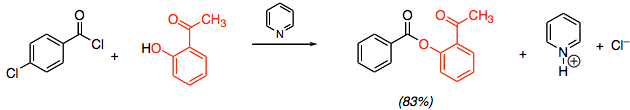
\includegraphics[scale=0.33]{esterfromcocl.png}\\
        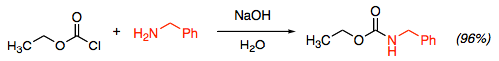
\includegraphics[scale=0.33]{amidefromcocl.png}
      \end{itemize}
    \item \textbf{Activating COOH $\rightarrow$ anhydride} by reacting with acid Cl or
      another anhydride:\\
      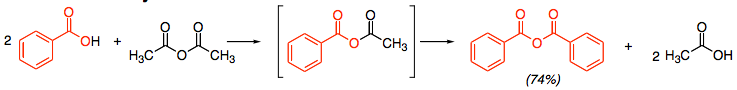
\includegraphics[scale=0.28]{forminganhydride.png}
      \begin{itemize}
      \item Anhydrides react similarly to acid Cl except eliminates a carboxylic acid
      \end{itemize}
    \end{itemize}
    
    \subsection{Acetals: carbonyl "protecting" groups}

    \begin{itemize}
    \item[] \img{acetal1.png}
    \item Formed via addition of alcohol to carbonyl
    \item Acid catalyzed, driven towards acetal by removal of water water. Reversible
      (hydrolyze with excess water and acid)
    \item \textbf{Stable in basic conditions, unstable in acidic}. Allows reversible
      conversion of carbonyl to diester, removing electrophilicity
    \item Examples
      \begin{itemize}
      \item Protecting carbonyl:\\
        \img{pr-cnyl.png}
      \item Protecting alcohol/di-alcohol:\\
        \img{pr-ol.png}
      \item First acid catalyzed acetal formation (H$^3$O$^+$ w/ protecting group), do
        reaction, then acid catalyzed hydrolysis in excess water
      \item 1,2-ethanediol protects carbonyl:
      \item Diethyl carbonate protects diol:
      \end{itemize}
    \end{itemize}

    \subsection{Preparation of organometallic reagents (using R-X)}

    \begin{itemize}
    \item X = halide (Mg, I)
    \item Reagents are very basic (reacts like R$^-$ b/c metal is electron-donating)
      and reactive (must be DRY)
    \item These nucleophiles are very strong and can participate in all the previous
      substitution/addition reactions
    \item \textbf{Grignard reagents (R-MgX):} Mg metal with alkyl halide, Mg inserted in
      between halide and carbon\\ 
      \img{grign.png}
    \item \textbf{Organolithium reagents (R-Li)}: Li + R-X\\
      \img{orglith.png}
    \item \textbf{Organocuprate reagents (R$_2$)-CuLi}: First make R-Li, then react with
      Cu-X twice\\
      \img{orgcup.png}
    \end{itemize}

    \subsection{Reactions with organometallic reagents (carbonyl $\rightarrow$ alcohol/ketone)}
    
    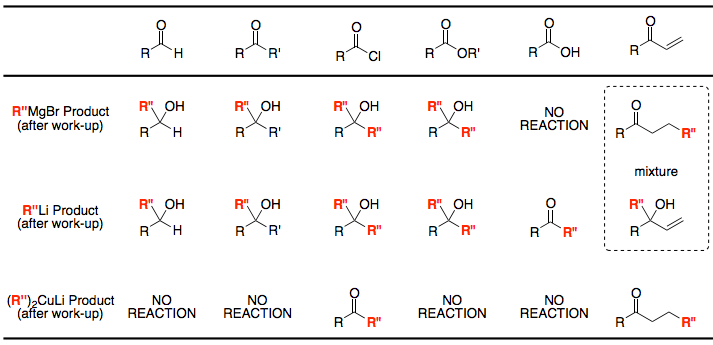
\includegraphics[scale=0.35]{metalsum.png}
    
    \begin{itemize}
    \item Electron-donating metal gives electrons to alkyl (forming R-C$^-$H$_2$) which
      acts as nucleophile
    \item Carboxylic-acid derivatives (have L-group) are substituted, aldehyde/ketone are reduced
    \item \textbf{Summary}: Use organocuprate to make 1,4-addition on Michael acceptor
      and converting acid chlorides to ketone. All else should use organolithium
    \item Don't forget acidic aqueous workup to protonate R-O$^-$ to alcohol
    \end{itemize}
    
    \subsection{Metal hydride addition (carbonyl $\rightarrow$ alcohol/amide)}
    
    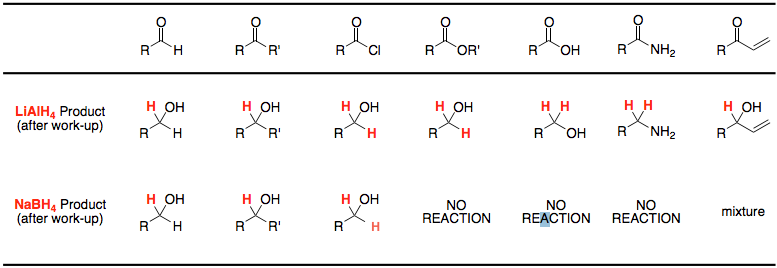
\includegraphics[scale=0.32]{hydride1.png}
    
    \begin{itemize}
    \item \textbf{Summary}: ALWAYS use LiAlH$_4$
    \item Electron-donating metal allows hydride (H$^-$) to act as nucleophile
    \item The Al metal is ``magical'':
      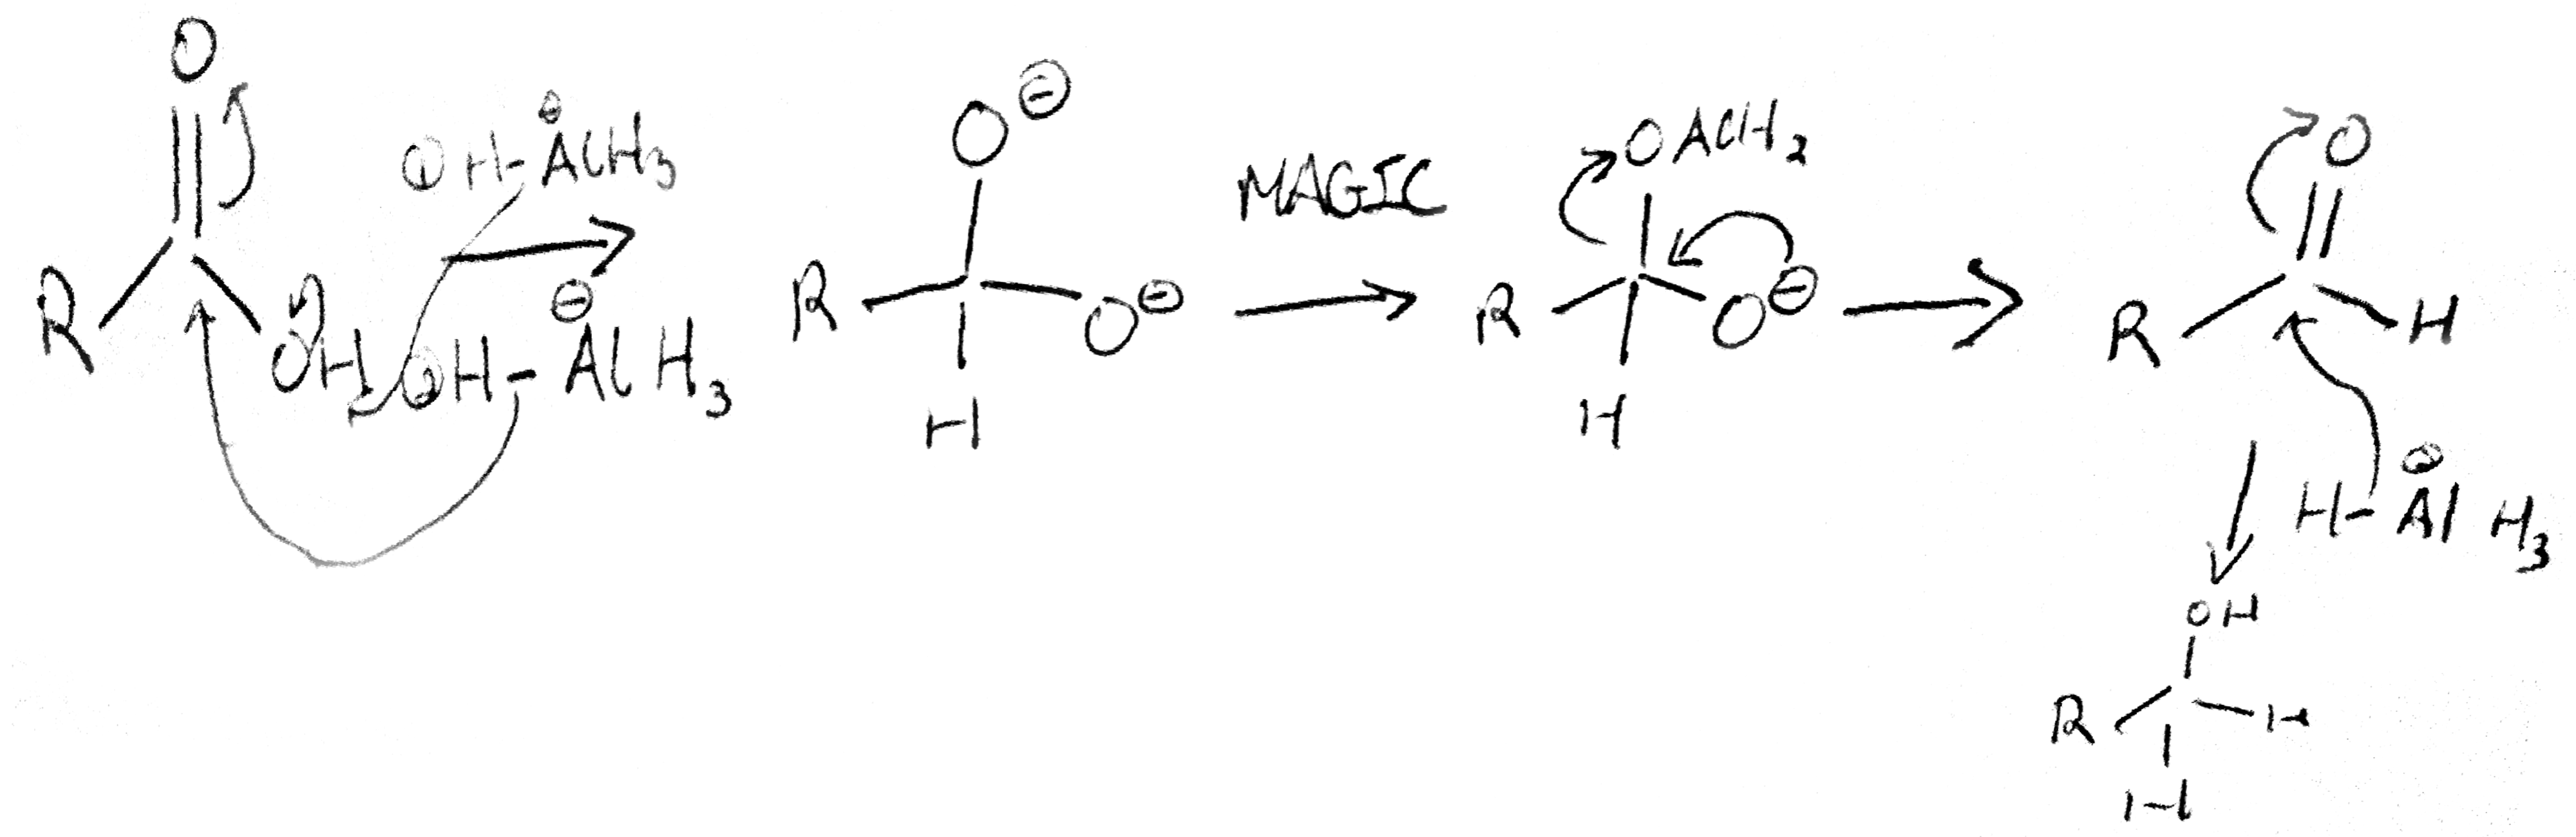
\includegraphics[scale=0.24]{hydr-cooh.png}
      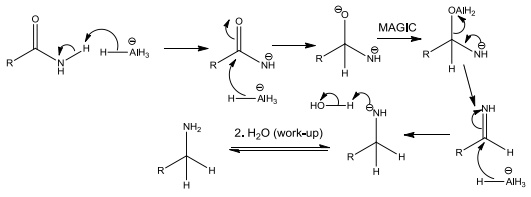
\includegraphics[scale=0.4]{hydr-amide.png}
    \item Nitriles can be hydrolyzed twice:
      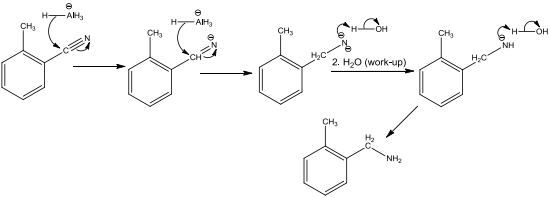
\includegraphics[scale=0.4]{hydr-nitrile.png}
    \end{itemize}
    
    \subsection{Chromium oxidants (alcohol $\rightarrow$ carbonyl)}
    
    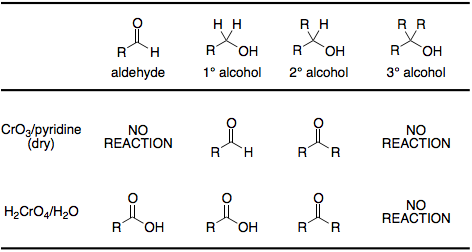
\includegraphics[scale=0.5]{chromiumox.png}
    
    \begin{itemize}
    \item \textbf{Summary}: Use H$_2$Cr$_2$O$_4$/H$_2$O fol all except making aldehyde
      from 1\dg alcohol
    \item Difference is due to hydration in aqueous conditions, thus any Cr oxidation rxn
      w/ aqueous conditions will react similar to H$_2$CrO$_4$/H$_2$O
    \item Reaction begins with carbonyl oxygen attacking CrO$_3$ to form chomate ester
      intermed, HCrO$_3^-$ is eliminated in E2 by any base
    \end{itemize}

    \subsection{Wittig reaction (carbonyl $\rightarrow$ alkene)}

    \begin{itemize}
    \item Wittig reagent (``ylide'') prepared from alkyl halide via phosphonium ion
      formation and deprotonanion w/ strong base\\
      \img{wittig1.png}
    \item Converts aldehydes and ketones into alkenes by replacing carbonyl double bond\\
      \img{wittig2.png}
    \item Reaction proceeds through 4-membered ring (``ylide'' carbon attacks carbonyl)
    \end{itemize}

    
    \subsection{Enolates}

    \begin{itemize}
    \item Properties of enolates:
      \begin{itemize}
      \item $\alpha$-carbon of ketones/aldehydes have weakly acidic H (resonance with
        carbonyl), deprotonation generates enolate
      \item Keto/enol forms equilibate, keto is lower energy and favored at neutral
      \item Tautomerization to enol catalyzed by base or acid
      \end{itemize}
    \item \textbf{Must use LDA} to forms enolate quantitatively and explicitly (prevent multiple alkylations):
      \img{enol1.png}
    \item Enolate can then act as nucleophile in substitution reactions with alkyl halides
      ($\alpha$-hydrogen $\rightarrow$ $\alpha$-substituted). However, this requires a strong
      base and can be avoided
    \end{itemize}
    
    \subsection{Acetoacetic ester synthesis(doubly-$\alpha$-proton $\rightarrow$
      $\alpha$-substituted carbonyl or $\beta$-ketoester)}

    \begin{itemize}
    \item[] \img{rcooet.png}
    \item $\beta$-ketoester stabilizes enolate and allows quantitative formation with mild
      bases ($^-$OEt/EtOH), enolate itself is also less reactive
    \item Synthetic equivalence - $\beta$-ketoester decarboxylation (note: requires
      $\beta$-carbonyl to COOH) generates same products as regular enolate attack 
    \item Multiple alkylations before decarboxylation possible (as is stopping and
      extracting 1,3-dicarbonyl)
    \end{itemize}

    \subsection{Malonic ester synthesis (doubly-$\alpha$-proton $\rightarrow$
      $\alpha$-substituted carboxylic acid or $\beta$-ketoester)}
    
    \begin{itemize}
    \item[] \img{malon1.png}
    \item Same as acetoacetic except during acidic workup one COOEt wil decarboxylate and
      \textbf{other will hydrolyze to carboxylic acid}
    \item Note: \textbf{any proton doubly-$\alpha$ to two anion stabilizing groups} can react similarly
    \end{itemize}

    \subsection{Aldol condensation (aldehyde $\rightarrow$ $\beta$-hydroxy or
      $\alpha$-$\beta$-unsaturated ketone)}

    \begin{itemize}
    \item[] \img{aldol.png}
    \item Aldehyde acceptor, aldehyde/ketone (enolate) donor
    \item \textbf{Crossed Aldol:} acceptor is aldehyde w/ \textbf{no $\alpha$-protons}
      and donor is \textbf{symmetrical} ketone or has protons on \textbf{only one
        $\alpha$-carbon} 
    \item Ketone acceptor possible \textbf{only in intramolecular ring forming} rxn
      \begin{itemize}
      \item Last step of Robinson annulation
      \end{itemize}
    \item Optional: $\beta$-hydroxyl group can be eliminated in E1cb reaction
      (1. Deprotonate 2. Eliminate $^-$OH L-group and form $\alpha$-$\beta$-unsaturated carbonyl)
    \item Reversible, acid and base catalyzed
    \end{itemize}

    \subsection{Claisen condensation (ketoester $\rightarrow$ 1,3-dicarbonyl)}

    \begin{itemize}
    \item[] \img{claisen.png}
    \item Ester acceptor, ester/ketone (enolate) donor
    \item \textbf{Crossed Claisen Donor}: \textbf{symmetrical ketone with 2/3
        protons on each $\alpha$-C} or \textbf{unsymmetrical with 1 H on one $\alpha$-C
        and 2/3 H on other} 
    \item \textbf{Crossed Claisen Acceptor}: \textbf{ester w/ no $\alpha$-C}
    \item Reversible, \textbf{$\beta$-ketoester must deprotonate to drive EQ}
    \end{itemize}

    \subsection{Michael addition ($\alpha$-$\beta$-unsaturated carbonyl $\rightarrow$ 1,5-dicarbonyl)}

    \begin{itemize}
    \item[] \img{michael1.png}
    \item Any good nucleophile (enolate, -CN, organometals, etc) attacks a Michael acceptor
      ($\alpha-\beta$-unsaturated carbonyl)
    \item Competes with normal carbonyl addition, increased by acid (protonated R=O$^+$H
      has res. struct. w/ + on $\beta$-carbon)
    \item Ketoester can be decarboxylated to give 1,5-dicarbonyl
    \item[] \img{michael2.png}
    \end{itemize}

    \subsection{Robinson Annulation}
    Forms bicyclic ring from cyclic enolate donor and Michael acceptor. Enolate adds in
    Michael addition, proton shifts form enolate on other side of Michael acceptor's
    carbonyl, enolate attacks in intramolecular aldol condensation.
    
  \end{scriptsize}
\end{multicols*}
\end{document}
%%% Local Variables: 
%%% mode: latex
%%% TeX-master: t
%%% End: 
